\section{Trigger requirements}
\label{sc:TriggerRequirements}

Events analyzed in this note were collected by the CMS experiment during the LHC
commissioning phase in December 2009. The majority of p-p collisions
recorded in this period were at $\sqrt{s}=900$~GeV, and a
smaller dataset was collected with $\sqrt{s}=2.36$~TeV. In order to
identify the collision candidates, we use the following
set of Level-1 ``technical'' triggers (TT), which are based on the Beam Scintillation
Counter (BSC) system~\cite{BSCTwiki}:

\begin{itemize}
\item{\bf At least one of the BSC MinBias TT:} require that at least one of
  the TT bits 40 or 41 fired. These triggers fire when there is a
  coincident activity in the forward and backward BSC detectors,
  indicating a collision candidate. Events collected by this triggers are found in the MinimumBias dataset.

\item{\bf None of the BSC beam halo triggers fired:} exclude events where any
  of TT bits 36, 37, 38, 39 fired. These triggers fire when the hits in
  the forward and backward BSC detectors are inconsistent in timing with
  originating from the collision.
\end{itemize}

\section{Data Samples}
\label{sc:DataSamples}

For the analysis presented in this note the
collision events were reconstructed using CMSSW\_3\_3\_6\_patch3 software release.
The events collected by the BSC triggers can be found in the ``MinimumBias'' dataset. 
We used the data sample in which the trigger selections
discussed in the previous section are already applied:
\begin{itemize}
\item /MinimumBias/BeamCommissioning09-BSCNOBEAMHALO-Jan23Skim-v1/RAW-RECO
\end{itemize}
Additionally, we require that the L1 BPTX trigger (TT bit 0) fired, which
indicates timing consistent with crossing of two proton bunches in the center of CMS detector. 
We also require that the ``HLT\_PhysicsDeclared'' bit is set, which (during December 2009 
data-taking) indicates that Tracker and Pixel detectors were up and 
running with stable beams in the accelerator. 

Out of all runs that are present in this data set and fulfill all
of the requirements listed above, the following runs were identified 
by the Physics Validation Team (PVT) group to have
problems in one or more sub-detectors (``bad'' runs): 123906, 123970, 123976, 123977, 
123978, 
% 123985, 
123987, 124006, 124230. 
Events collected during these runs are excluded
from this analysis, unless it is stated otherwise.

After excluding the bad runs listed above, the set of runs listed in
Tab.\ref{tab:goodruns} is used for the analysis presented in this
note. 

\begin{table}[h]
  \begin{center}
    \begin{tabular}{|c|c|c|c|}
      \hline
      Run Number      & Beginning LumiSection  & Ending LumiSection   \\\hline\hline
      123596              & 2   & 9999\\ 
%       123615              & 70 & 9999\\
      123732              & 62 & 109\\
      123815              & 8   & 9999\\
      123818              & 2   & 42\\
      123908              & 2   & 12\\
      124008              & 1   & 1\\
      124009              & 1   & 68\\
      124020              & 12 & 94\\
      124022              & 66 & 179\\
      124023              & 38 & 9999\\
      124024              & 2   & 83\\
      124025              & 5   & 13\\
      124027              & 24 & 9999\\
      124030              & 2   & 9999\\
      124120              & 1   & 9999\\
      \hline    
    \end{tabular}
    \caption{List of runs and corresponding lumisections that were analyzed in this note. For some of
      the runs only a certain range of lumisections is considered to be
      good for analysis. If the ending lumisection is labelled as 9999 it
      means that the run was good until its end.}
    \label{tab:goodruns}
  \end{center}
\end{table}

Due to technical difficulties with the reconstruction of raw data, runs 123615 and 123985 were missing
from the above mentioned dataset. The approximate integrated luminosity collected during the whole data taking period 
(including periods with physics declared bit not set and runs with identified detector problems) 
is 15~$\mu\mbox{b}^{-1}$. More detailed informations can be found at~\cite{ref:LumiWithHF}. 

\subsection{Monte Carlo simulation}

The collision data events considered in this analysis are compared with
{\sc pythia} simulations of Minimum Bias collisions which are processed
with {\sc GEANT-4} simulation of the CMS detector. Simulated events are
then reconstructed using CMSSW\_3\_3\_6\_patch3. The Monte Carlo samples used in
this analysis are:
\begin{itemize}
\item 900 GeV Mininum Bias: /MinBias/Summer09-STARTUP3X\_V8P\_900GeV-v1/GEN-SIM-RECO 
\item 2360 GeV Mininum Bias: /MinBias/Summer09-STARTUP3X\_V8O\_2360GeV-v1/GEN-SIM-RECO
\end{itemize}

For the comparisons of data with Monte Carlo we require that simulated
events pass the BSC Minimum Bias trigger selections (TT bits 40 and
41). Additionally, any further event selection criteria described in Section~\ref{sec:event_selection}.
are applied to both data and simulation.

\section{Event Selection and Cleaning of Anomalous Noise}
\label{sec:event_selection}
In this section we describe the event selection, based on reconstructed quantities, 
which is used to both identify good collision candidate events and to remove instrumental 
and beam related noise sources. We present the algoritms used to 
identify channels affected by anomalous noise in the calorimeters and summarize 
the effect of the noise cleaning on the $\etmiss$ distribution.

\subsection{Removal of scraping events}
\label{sc:scrapingFilter}

During the LHC commissioning phase, it was observed that
in some bunch crossings there was a anomalously large occupancy in the
pixel detector, which resulted in a large number of reconstructed fake
tracks. These events were identified as being the result of beam
particles traversing the pixel detector longitudinally. We reject this
type of events by requiring that the fraction of ``high-purity'' tracks in
all events with more than 10 tracks is greater than 25\%, following the 
recommendation from PVT group.

\subsection{Vertex selection}
In order to further constrain the event selection to identify the
collision events, a selection based on
the reconstructed primary vertex properties is implemented. 
The selection is based on the following quantities: vertex $\chi^2$, number of
degrees of freedom (NDF) of the vertex, and vertex $z$ coordinate.
%number of tracks which contributed to the vertex reconstruction
%with a weight $>0.5$, 
Figure~\ref{fig:vertex_selection_1} and~\ref{fig:vertex_selection_2} shows
the distributions of vertex $z$ coordinate, vertex $\chi^2$ 
and vertex NDF in data compared to simulation; distributions are shown for events 
that pass all the selections described so far (excluding filter for scraping events) 
with the additional requirement to have at least 2 tracks which 
contributed to the vertex reconstruction with a weight $>0.5$. 

We implement the official recommendation from the tracking group 
to identify collision events by requiring:
\begin{itemize}
\item vertex $\chi^2\ne0$, NDF$\ne0$ and contains more than 0 tracks
  associated to it, to reject fake vertices (``isFake()'' bit set to false)
\item NDF is greater than 4
%\item number of tracks with weight$>0.5$ is greater than 3.
\item vertex $|z|\leq 15$~cm
\end{itemize}

\begin{figure}[h]
 \centering
 \begin{tabular}{ll}
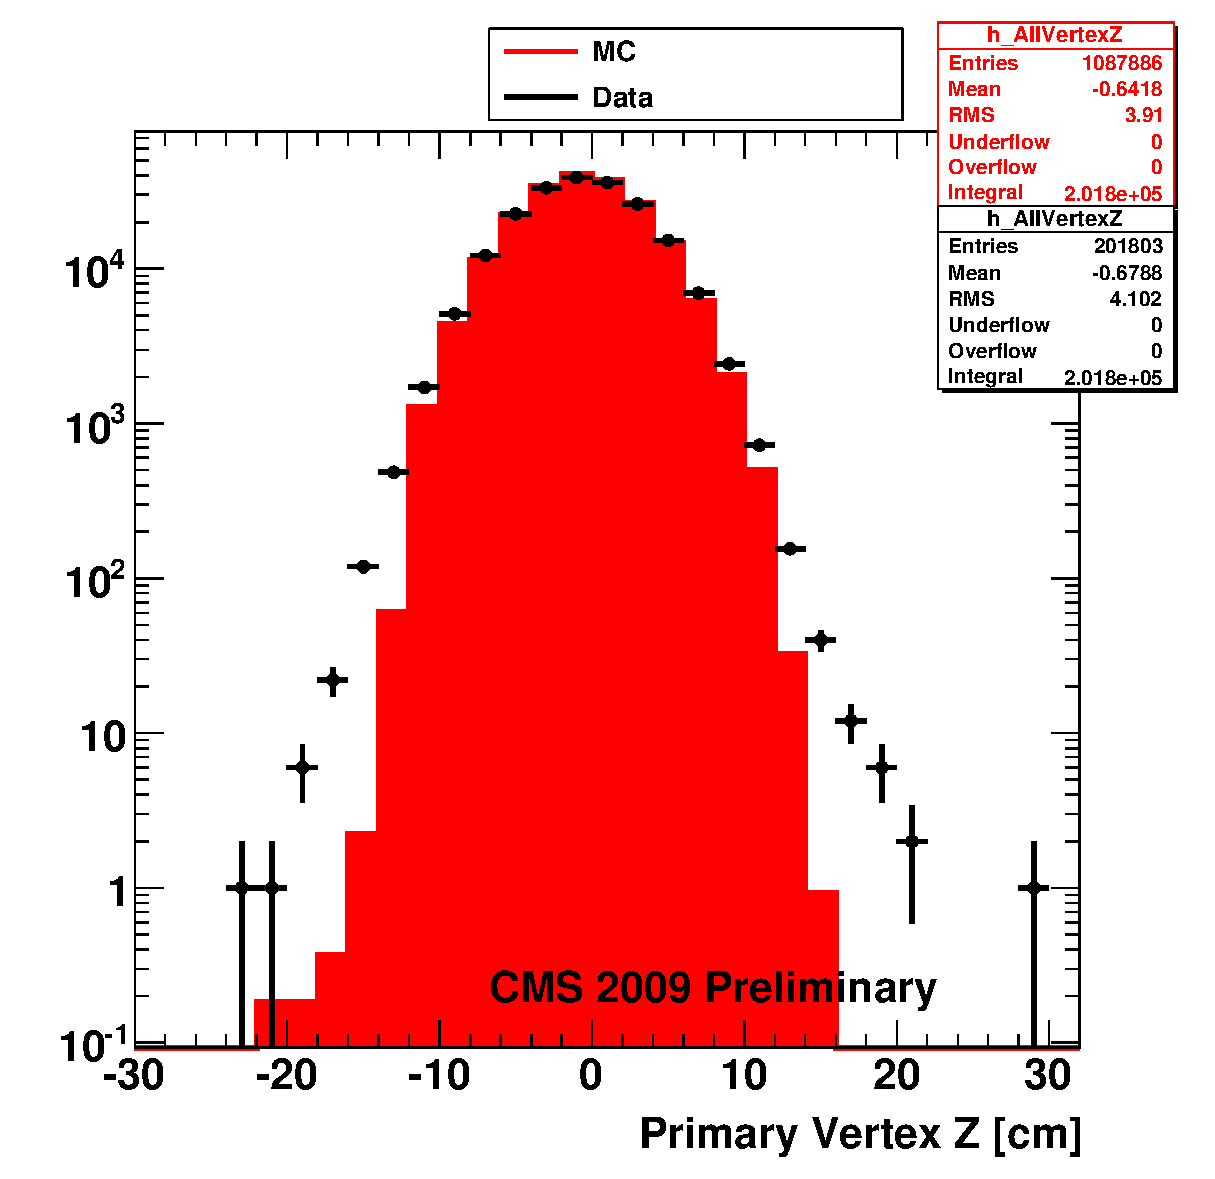
\includegraphics[width=0.5\textwidth]{plots_EventSelection/h_AllVertexZ_log.eps}&
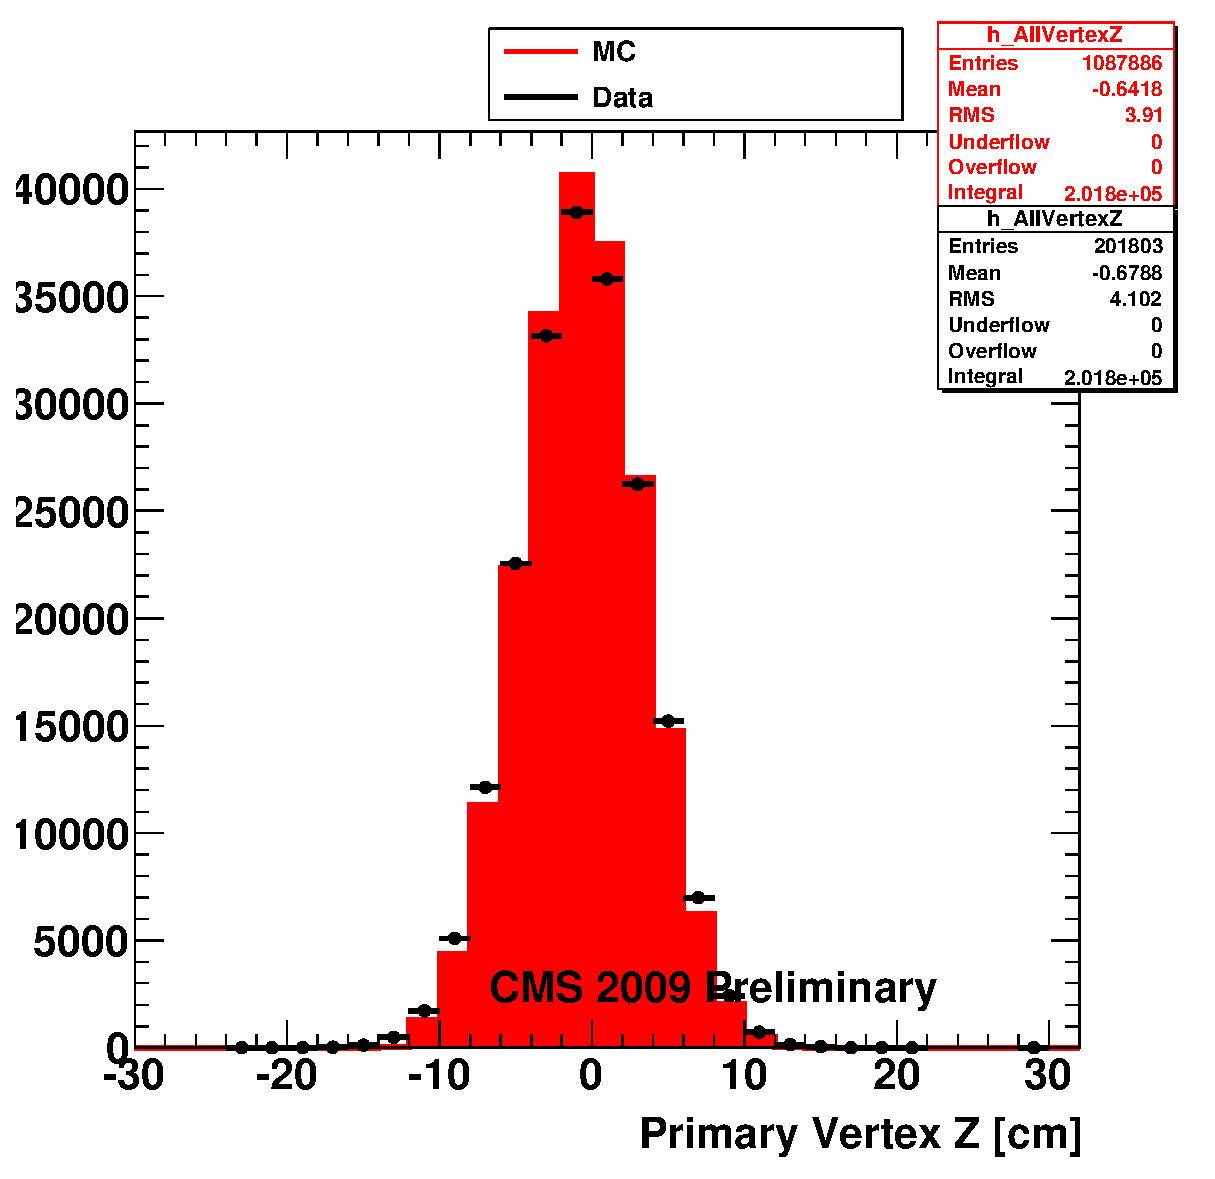
\includegraphics[width=0.5\textwidth]{plots_EventSelection/h_AllVertexZ_linear.eps}\\
 \end{tabular}
\caption{Comparison of the distribution of the event primary vertex $z$
  position between data and Monte Carlo simulation, in log (left) and
  linear (right) scales at 900 GeV.}
\label{fig:vertex_selection_1}
\end{figure}

\begin{figure}[h]
 \centering
 \begin{tabular}{ll}
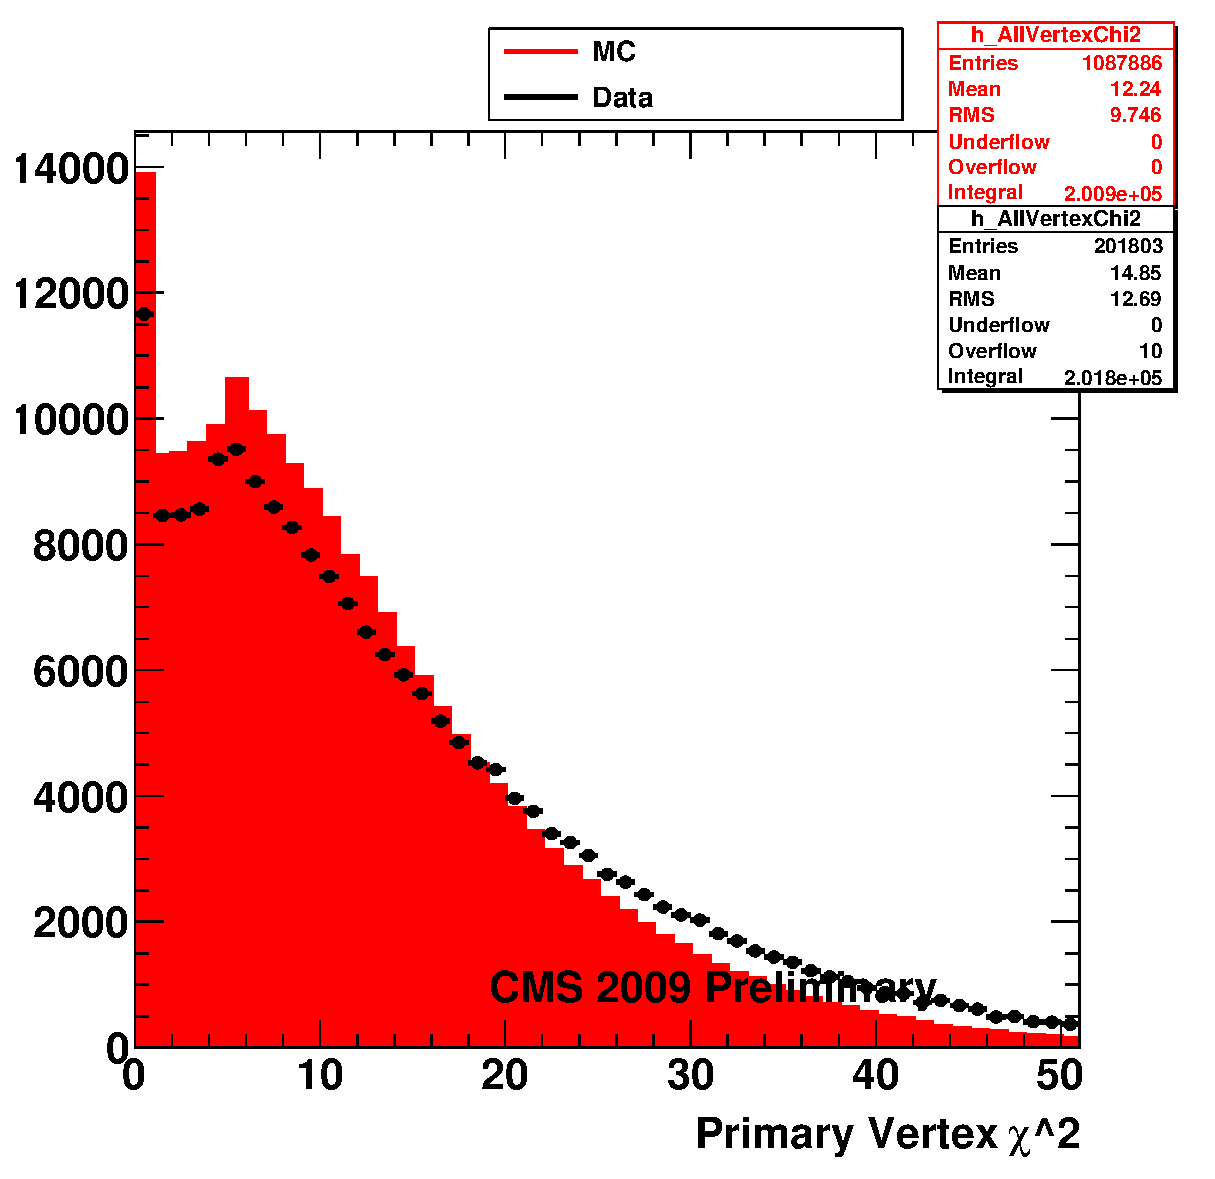
\includegraphics[width=0.5\textwidth]{plots_EventSelection/h_AllVertexChi2.eps}&
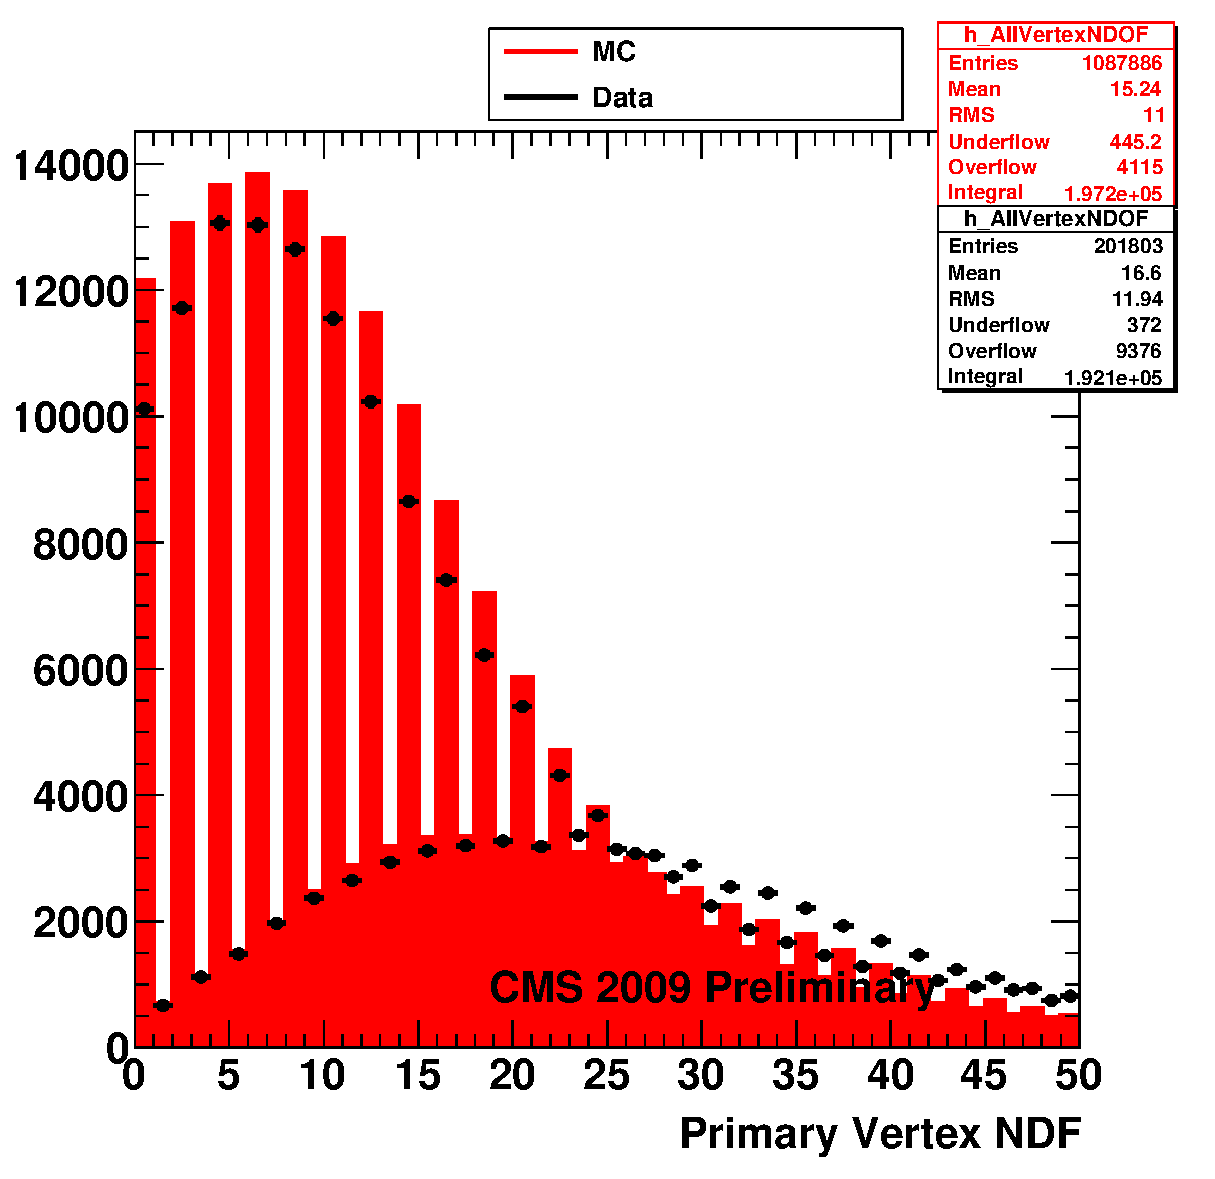
\includegraphics[width=0.5\textwidth]{plots_EventSelection/h_AllVertexNDF.eps}\\
 \end{tabular}
\caption{Comparison of the distribution of the event primary vertex
  $\chi^2$ and NDF between data and Monte Carlo simulation at 900 GeV. }
\label{fig:vertex_selection_2}
\end{figure}

\subsection{HCAL anomalous noise} \label{sec:HCALNoise}
Commissioning studies of the CMS hadronic calorimeter performed 
during past test beam, cosmic, and single beam runs have 
identified anomalous noise (i.e. not due to regular 
electronic/pedestal noise) that can be grouped in two categories~\cite{Chatrchyan:1225105}:
\begin{itemize}
\item{\bf HB/HE Anomalous Noise} The source of the anomalous noise in the HCAL 
barrel (HB) and endcap (HE) subdetectors is due to characteristics 
of the hybrid photo-diodes (HPDs), used to convert the scintillator light into 
an electrical output, and the readout boxes (RBXs) that they lie within.
Such atypical signals can be categorized 
in i) Ion Feedback Noise (typically affecting 1-2 channels in one HPD), ii) HPD Noise 
(coherent affecting up to 18 channels in one HPD), iii) RBX Noise 
(coherent noise affecting up to 72 channels in one RBX unit);
\item{\bf HF Photo-Multipliers (PMT) Window Hits} An energetic charged particle, directly 
impinging upon the window of an HF PMT, can produce an abnormally large apparent 
energy signal for a single HF channel (the one associated to that PMT). 

Such process can be briefly explained as follows.
A relativistic charged particle, when traversing the PMT window glass, 
generates Cerenkov light in the usual Cerenkov cone. Cerenkov light can initiate the liberation 
of photoelectrons depending on the incidence angle of the particle with respect to window/photocathode geometries, 
whether the light falls within the acceptance range of the PMT photocathode in terms of wavelength, 
and the photocathode efficiency. The photoelectrons then produce a potentially large and fake signal as if it 
is a photodetection of an external event.

Such interactions can possibly happen due to beam halo muons, punch-through particles generated 
from the particle showers inside HF absorber or later showering pions.
Studies to estimate which of these processes is dominating in this data are still ongoing.
\end{itemize}

The presence of such atypical signals was also confirmed in recent 
2009 collision data, sometimes resulting in large unphysical $\etmiss$ in the event. 
Observations indicate that large unphysical HCAL-related $\etmiss$ 
in Minimum Bias events is mostly due to energy reconstructed in HF, 
while in only few cases the energy unbalance is due to HB/HE noise events. 
This can be explained by considering that HF PMT window hits 
are related with the beam activity (for example beam halo muons hitting the PMT window), 
while HB/HE noise (HPD and RBX noise) occurs at random time and it is 
uncorrelated with the beam activity. Therefore the probability of overlap 
of an HB/HE noise event with a collision event is relatively small.

The approach used in this note to identify anomalous noise events in HCAL is described below.

\begin{itemize}
%
\item{\bf HBE/HE noise events} A set of algorithms have been developed by the HCAL group to 
identify and address these types of problems in the data. The methods have been tested on cosmic muon data, 
dedicated calorimeter noise data, and single beam data collected at CMS in 2008, 
as described in~\cite{Chatrchyan:1225105},~\cite{HCALNoiseTwiki}.  

The commissioning of the noise identification algorithms with collission data is still 
ongoing and some of the variables, discriminating between signal and noise, rely on the proper 
timing alignment of the HCAL detector, which is not fully understood at the startup.
Therefore, taking also into consideration that the probability of overlap between such noise and 
collision events is observed to be small (for example with respect to HF anomalous noise), 
it has been decided to follow a conservative approach and don't apply any cleaning for HB/HE noise 
at this early stage of the analysis.
%
\item{\bf HF PMT window hits} PMT windows hits within HF channels are tagged by comparing 
the energies reconstructed from long (L) and short (S) fibers with the same ($\eta$,$\phi$) values. 
Infact, a particle hitting directly a PMT would produce a large apparent energy only in one channel 
(i.e. either the one connected to long or short fiber) and none in the other.

Given a pair of adjacent long and short fiber channels at the same ($\eta$,$\phi$) value 
with energies $E^\text{L}$, $E^\text{S}$, respectively, the fiber channels are flagged as noisy if 
(a) the transverse energy measured in the HF tower ($E_\text{T}=E_\text{T}^\text{L}+E_\text{T}^\text{S}$) is at least 5~GeV, 
and (b) the energy ratio $R$, defined as:
%
\begin{equation}
R = \frac{E^\text{L} - E^\text{S}}{E^\text{L} + E^\text{S}}
\end{equation}
%
is greater than 0.99 (PMT hit associated to the long fiber) 
or smaller than -0.8 (PMT hit associated to the short fiber).
Some of the HF fiber channels (3 long fibers and 5 short fibers) 
were masked in the calotower reconstruction since identified as hot channels. 
HF towers corresponding to those ($\eta$,$\phi$) regions are not considered for 
the cleaning procedure.
 
Figure~\ref{fig:hf_noise_ET_vs_R} shows the scatter distribution of $E_\text{T}$ vs $R$, 
for both data and MC, after applying all the event selection criteria except 
the HF filter itself. The HF noise channels can be identified by 
large $E_\text{T}$ values and $R$ values close to -1 or 1, 
inconsistent with MinBias MC assumption.

%In this study, if at least one HF fiber channel is flagged by this algorithm, 
%the event is simply rejected from the analysis. No attempt to clean the event, 
%by correcting the high level objects (such as $\etmiss$ or $\sumet$), 
%is performed at this stage of the analysis. 

%
%
\begin{figure}[h!]
 \centering
 \begin{tabular}{ll}
  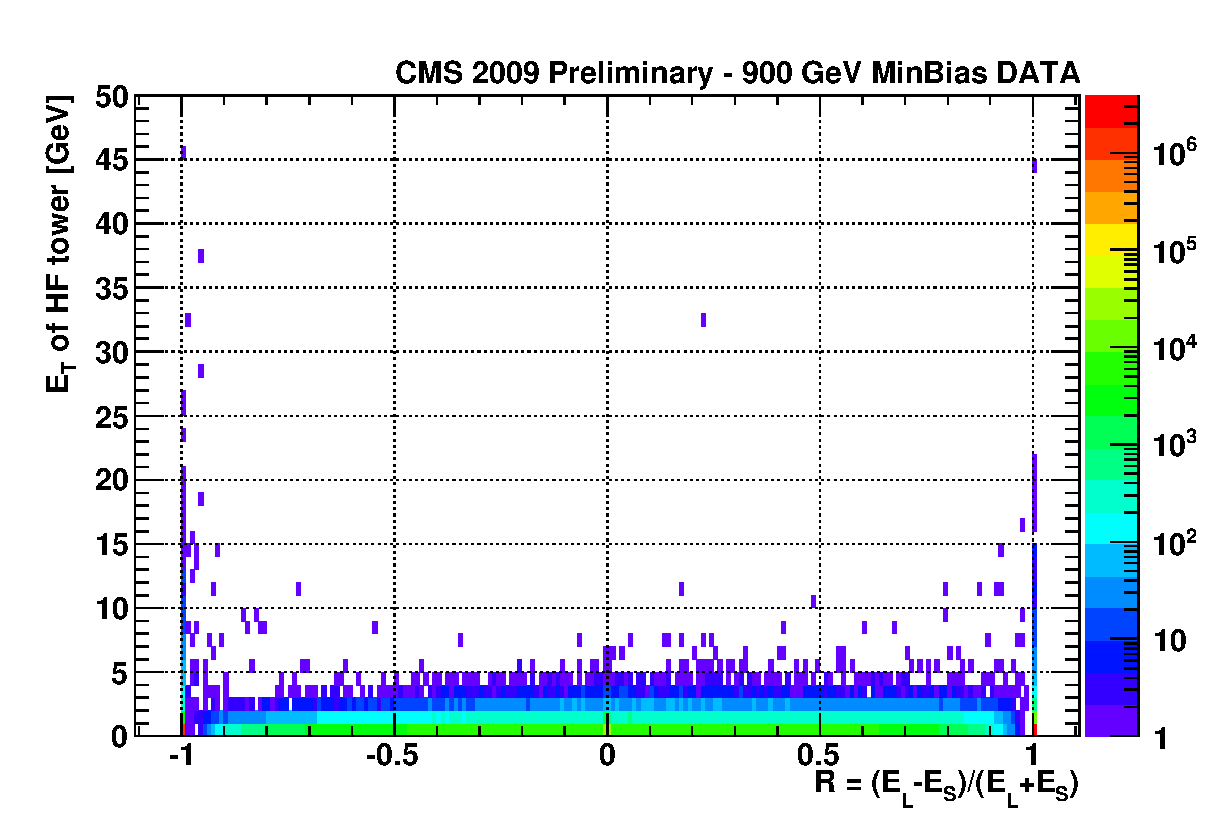
\includegraphics[width=0.5\textwidth]{plots_hcalnoise/hf_towerET_vs_ratio_DATA.eps} &
  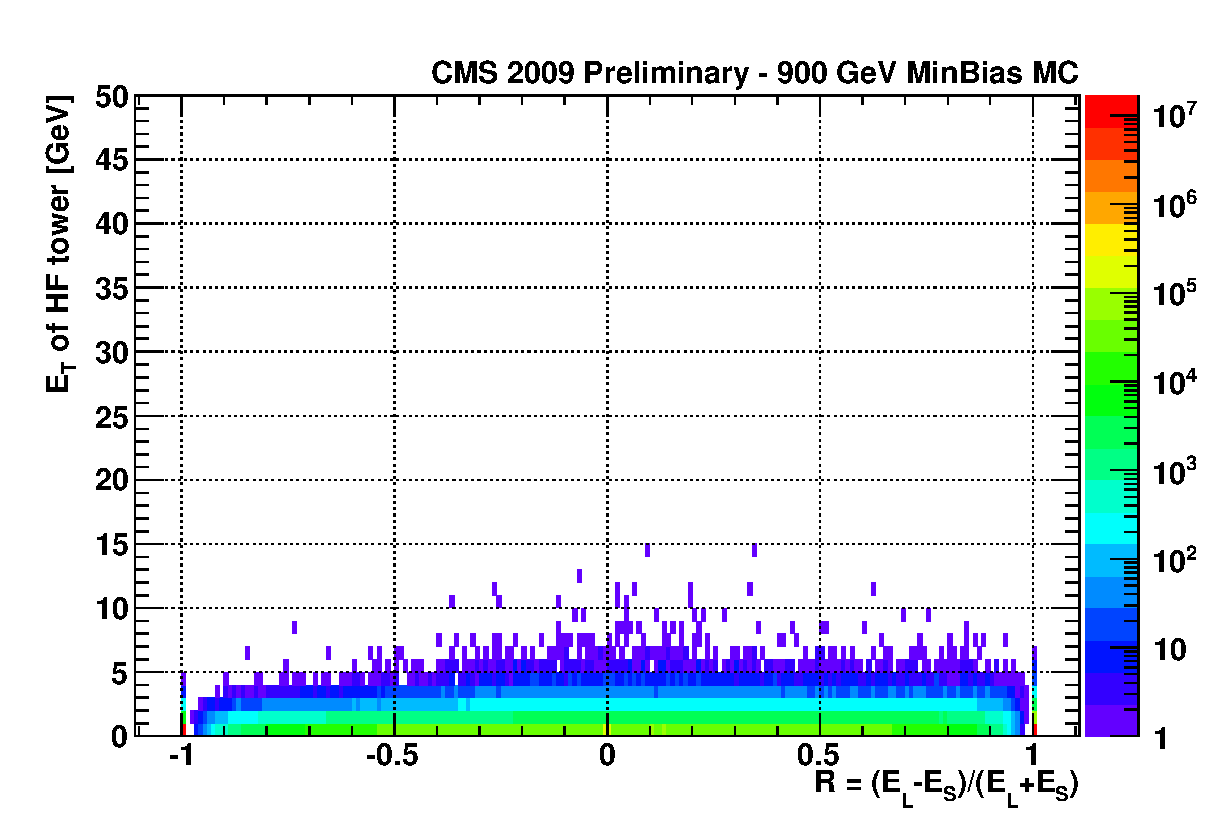
\includegraphics[width=0.5\textwidth]{plots_hcalnoise/hf_towerET_vs_ratio_MC.eps} \\
 \end{tabular}
\caption{\small Scatter distribution of transverse energy in HF tower versus energy ratio $R$ for both data 
(Left) and MC (Right), after applying all the event selection criteria except the HF filter itself. 
Plots are filled for each HF tower if either $E^\text{L}>1.2$~GeV or $E^\text{S}>1.8$~GeV (to cut the pedestal noise).
\label{fig:hf_noise_ET_vs_R}}
\end{figure}
%
%
\end{itemize}

\subsection{ECAL anomalous noise} \label{sec:ECALNoise}

A set of events with unphysical characteristics in the barrel of the ECAL
calorimeter (EB) was observed during the initial analysis of the
$\sqrt{s}=900$~GeV data collected at CMS. These events are typically 
characterized by energy deposits in a single, isolated ECAL crystal (``spike''
crystal), while the crystals in the immediate neighborhood of the spike
crystal contain little or no energy.  
This kind of energy deposit is incompatible with energy 
deposits due to a real photon or electron,
given the Moliere radius and crystal sizes in ECAL. 
In addition, preliminary studies show that, usually, the ECAL 
spikes are isolated from hadronic activity and there are 
no tracks pointing to them. Since the presence
of a spike crystal in an event with no $\etmiss$ may appear to have
energy imbalance in the transverse plane, it is crucial to identify this
type of noise and efficiently remove it.

Unlike the HCAL anomalous noise described in the previous section, ECAL
spike events were not identified in the data taken before the collision runs
in December 2009 (however, it has been confirmed that spike events 
have occurred also during previous cosmic runs). The study to understand the
source of ECAL spike events and to efficiently identify them is
currently ongoing~\cite{ref:ECALSpikes1},~\cite{ref:ECALSpikes2}. The approach we have taken to identify the ECAL
spikes in this analysis is described below.

\begin{figure}[h]
 \centering
 \begin{tabular}{ll}
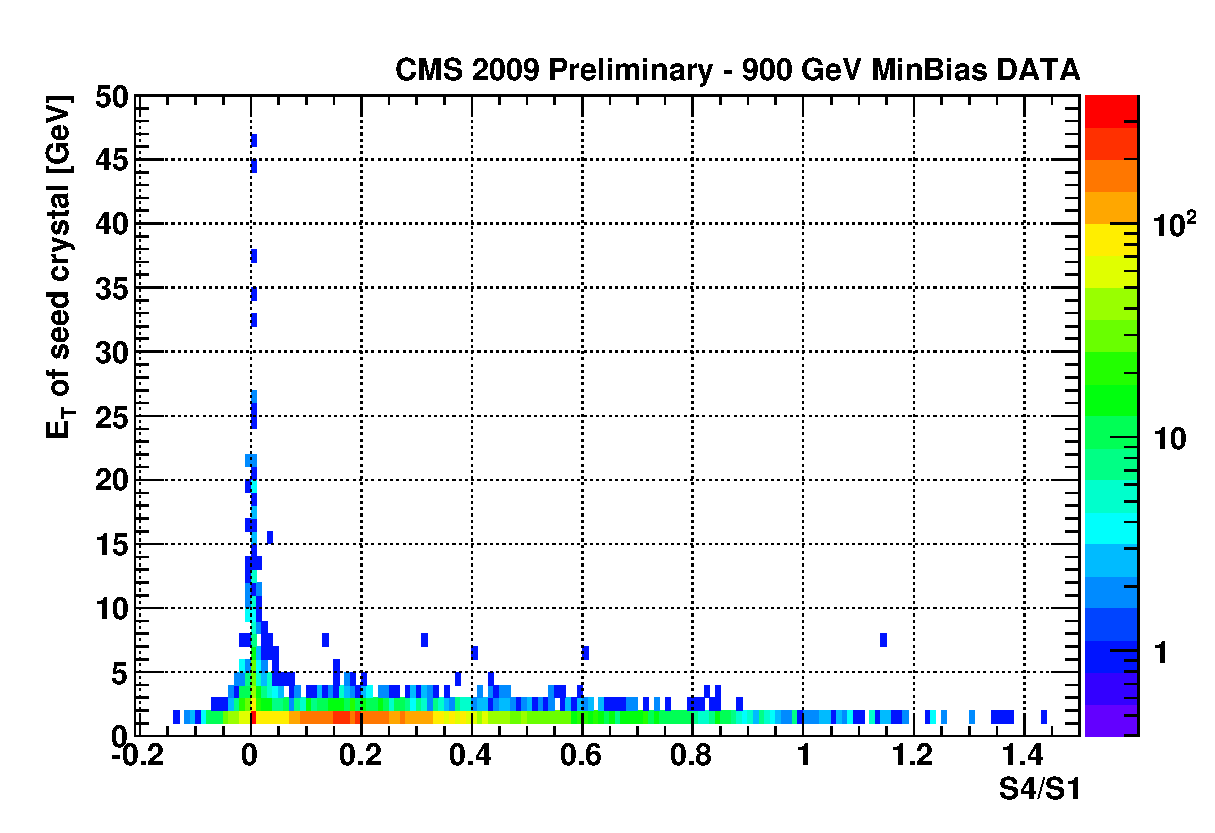
\includegraphics[width=0.5\textwidth]{plots_ecalnoise/ECalSeedET_Vs_S4_DATA900GeV.eps}&
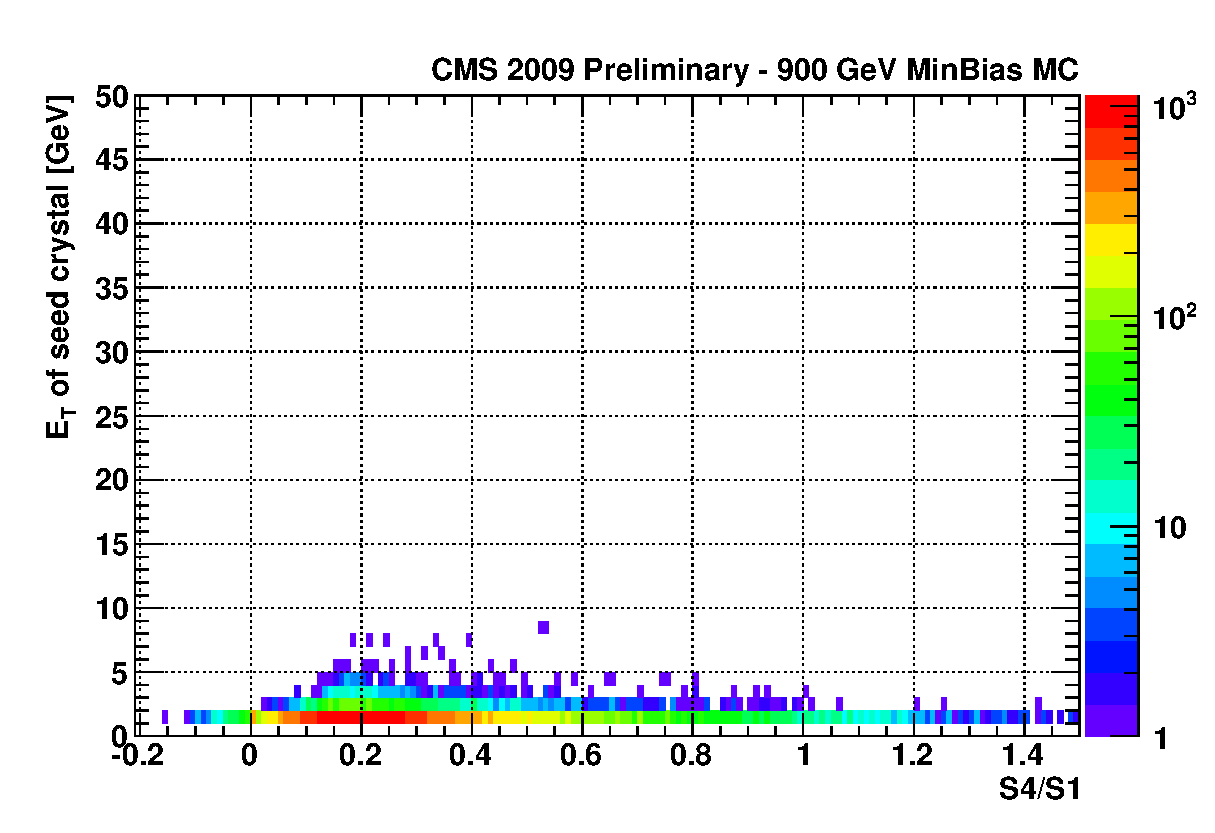
\includegraphics[width=0.5\textwidth]{plots_ecalnoise/ECalSeedET_Vs_S4_MC900GeV.eps}\\
 \end{tabular}
\caption{Distributions of the $S4/S1$ in 900 GeV data and Monte Carlo
  for ECAL barrel. Distributions are shown for events that pass all
  selections described in previous sections, except the EB cleaning itself.}
\label{fig:ecal_noise_1}
\end{figure}

The total energy deposited in the crystals in the immediate
neighbourhood of the spike is expected to be small compared to the
energy of the spike crystal itself. Therefore, the ratio of energy
deposited in the neighbourhood of the spike crystal to the energy
measured in the spike itself is expected to be very small, provided 
that the occupancy in the ECAL is low.

The algorithm for identification of spikes proceedes as follows: 
i) we use the ``hybridSuperClusters'' algorithm to reconstruct the ECAL
clusters in EB, ii) we identify the possible spike candidates as the cluster seeds  
(the seed is the crystal with maximum energy inside a given cluter),
iii) we then calculate the quantity $S4/S1$, where $S4$ is defined as 
a sum of energies deposited in four crystals that share an edge with the seed, 
and $S1$ is the energy measured in the seed crystal, iv) we identify a spike
if $E_\text{T}^\text{seed}>5$~GeV and $S4/S1<0.05$.
The scatter distributions of $E_\text{T}^\text{seed}$ vs $S4/S1$ in data and
simulation for $\sqrt{s}=900$~GeV are shown in Fig.\ref{fig:ecal_noise_1}. 

%In this analysis we consider the quantity
%$S4/S1$, where $S4$ is defined as a sum of energies deposited in four
%crystals that share an edge with the spike, and $S1$ is the energy
%measured in the spike crystal. 
%The distributions of $S4/S1$ in data and
%simulation for 900 GeV are shown in Fig.\ref{fig:ecal_noise_1}. The
%``hybridSuperClusters'' algorithm was used to reconstruct the ECAL
%clusters. A distinct set of events in data can be observed with $S4/S1$
%values below 0.05 for events with $E_\text{T}>5$~GeV in the spike
%crystal. This feature is not observed in the Monte Carlo
%simulation. Therefore, we identify spike events by requiring that an
%ECAL crystal has $E_\text{T}>5$~GeV and $S4/S1<0.05$.

\subsection{Selection efficiencies and noise cleaning}

Tables~\ref{tab:selectionefficiency_900},\ref{tab:selectionefficiency_2360}
summarize the number of events after each set of baseline event selection
criteria (excluding anomalous noise cleaning), 
as well as their efficiencies in data and simulation, both at 900 GeV and 2360 GeV. 
After the baseline selection, the events cointaining one or more channels 
affected by anomalous noise are cleaned as described below.
 
The channels with anomalous noise in HF and EB are identified by the algorithms 
described, respectively, in Section and~\ref{sec:HCALNoise} and~\ref{sec:ECALNoise}.
No cleaning for EE channels is applied, since no anomalous noise has been observed 
so far in the ECAL endcaps. No algorithm to clean HB/HE anomalous noise is applied 
at this stage of the analysis, as described in Section~\ref{sec:HCALNoise}.
For events passing the baseline selection criteria, Table~\ref{tab:noiseCleaning} shows the number of
channels identified by noise cleaning algorithms in EB and HF and the average number of flagged channels 
per event in data and Monte Carlo, both at 900 GeV and 2360 GeV.
HF (EB) channels are flagged in the data at a rate of approximately 2 channels (1 channel) 
every $10^3$ events. The anomalous noise is not simulated in the Monte Carlo. In the simulation 
order of 1 channel every $10^5$ events is incorrectly flagged as HF noise channel.
With the current MC statistics available no EB channels are incorrectly flagged 
as anomalous noise in the simulation.

The event cleaning is performed by removing the energy of the 
individual noisy channels (energy of crystals in EB, and either energy in 
long or short fibers in HF) from the $\etmiss$ and $\sumet$ reconstruction.
Figure~\ref{fig:calometAfterCuts} shows the effect of the EB and HF 
noise cleaning on the $\etmiss$ distribution.
The algorithms described above can be seen to reject the majority of
large $\etmiss$ events in this Minimum Bias dataset (given that, currently, the occupancy 
of EB and HF calorimeters is low), including the shoulder in $\etmiss$ distribution around 16-20~GeV.
The noise cleaning criteria will have to be improved in order to work properly 
also in an high occupancy environment (for example, QCD jet events at $\sqrt{s}=7$~TeV).
Studies on this topic are ongoing within the CMS Collaboration.

\begin{table}[!ht]
  \begin{center}
    \begin{tabular}{|c|c|c|c|}
      \hline
      Selection (900 GeV DATA) & Number of Events  & Relative Efficiency & Absolute Efficiency\\
      \hline\hline
      BSC Triggers + PhysDecl  & 369517            & -                   & -      \\ 
      BPTX Trigger             & 321678		   & 0.870               & 0.870  \\
      Good Run List            & 215286		   & 0.669		 & 0.583  \\
      Good Primary Vertex      & 164704		   & 0.765		 & 0.446  \\
      Scraping Events Removal  & 164703		   & $\approx$ 1	 & 0.446  \\
      \hline
      \hline
      \hline
      \hline
      Selection (900 GeV MC)   & Number of Events  & Relative Efficiency & Absolute Efficiency\\
      \hline\hline
      no cut                   & 1761550           & -                   & -      \\ 
      BSC Triggers	       & 1175201	   & 0.667               & 0.667  \\ 
      Good Primary Vertex      & 866821		   & 0.738		 & 0.492  \\
      Scraping Events Removal  & 866821		   & 1			 & 0.492  \\
      \hline
  \end{tabular}
    \caption{Number of events passing each selection criteria and
      the efficiencies of the various selections applied for data and Monte Carlo at $\sqrt{s}=900$~GeV. 
      The requirements of Physics Declared bit set, the beam crossing (BPTX trigger) and the Good Run selection 
      are not applied on MC.}
    \label{tab:selectionefficiency_900}
  \end{center}
\end{table}


\begin{table}[!ht]
  \begin{center}
    \begin{tabular}{|c|c|c|c|}
      \hline
      Selection (2360 GeV DATA) & Number of Events  & Relative Efficiency & Absolute Efficiency\\
      \hline\hline
      BSC Triggers + PhysDecl  & 14559             & -                   & -      \\ 
      BPTX Trigger             & 11868		   & 0.815               & 0.815  \\
      Good Run List            & 11868		   & 1		         & 0.815  \\
      Good Primary Vertex      & 9685		   & 0.816		 & 0.665  \\
      Scraping Events Removal  & 9685		   & 1			 & 0.665  \\
      \hline
      \hline
      \hline
      \hline
      Selection (2360 GeV MC)   & Number of Events  & Relative Efficiency & Absolute Efficiency\\
      \hline\hline
      no cut                   & 375000            & -                   & -      \\ 
      BSC Triggers	       & 252058		   & 0.672               & 0.672  \\ 
      Good Primary Vertex      & 191785		   & 0.761		 & 0.511  \\
      Scraping Events Removal  & 191785		   & 1			 & 0.511  \\
      \hline
  \end{tabular}
    \caption{Number of events passing each selection criteria and
      the efficiencies of the various selections applied for data and Monte Carlo at $\sqrt{s}=2360$~GeV. 
      The requirements of Physics Declared bit set, the beam crossing (BPTX trigger) and the Good Run selection 
      are not applied on MC.}
    \label{tab:selectionefficiency_2360}
  \end{center}
\end{table}



\begin{table}[!ht]
  \begin{center}
    \begin{tabular}{|c|c|c|c|c|}
      \hline
                                   & 900 GeV DATA  & 2360 GeV DATA & 900 GeV MC & 2360 GeV MC \\
      \hline\hline
      $N_{sel}$                    & 164703           &     9685          &      866821         &      191785            \\
      \hline\hline
      N. EB flagged channels             & 158              & 14                 & 0                   & 0                      \\
      N. EB flagged channels / event     & $9.6 \times 10^{-4}$ & $1.4 \times 10^{-3}$ & 0                   & 0                      \\
      \hline\hline
      N. HF flagged channels             & 351              & 28                 & 12                  & 7                      \\
      N. HF flagged channels / event     & $2.1 \times 10^{-3}$ & $2.9 \times 10^{-3}$ & $1.4 \times 10^{-5}$  & $3.6 \times 10^{-5}$     \\
      \hline\hline
  \end{tabular}
    \caption{Number of events passing baseline selection criteria ($N_{sel}$), number of EB and HF channels flagged by noise cleaning algorithms 
and fraction of flagged cells per event for data and Monte Carlo, both at 900 GeV and 2360 GeV.}
    \label{tab:noiseCleaning}
  \end{center}
\end{table}



%It can be seen from 
%Tab.~\ref{tab:selectionefficiency_data} that the number of events
%rejected by the ECAL/HCAL noise identification algorithms described
%above is relatively small. However, since this
%events can create an apparent imbalance in transverse energy, which can
%also populate the tails of distributions, it is crucial to identify
%them. 
%Fig.~\ref{fig:calometAfterCuts} shows how the
%$\etmiss$ distribution changes after removing the events with ECAL and HF
%noise. The algorithms described above can be seen to reject the majority of
%``large'' $\etmiss$ events, including the shoulder in $\etmiss$
%distribution around 16-20~GeV.


\begin{figure}[h!]
 \centering
 \begin{tabular}{ll}
  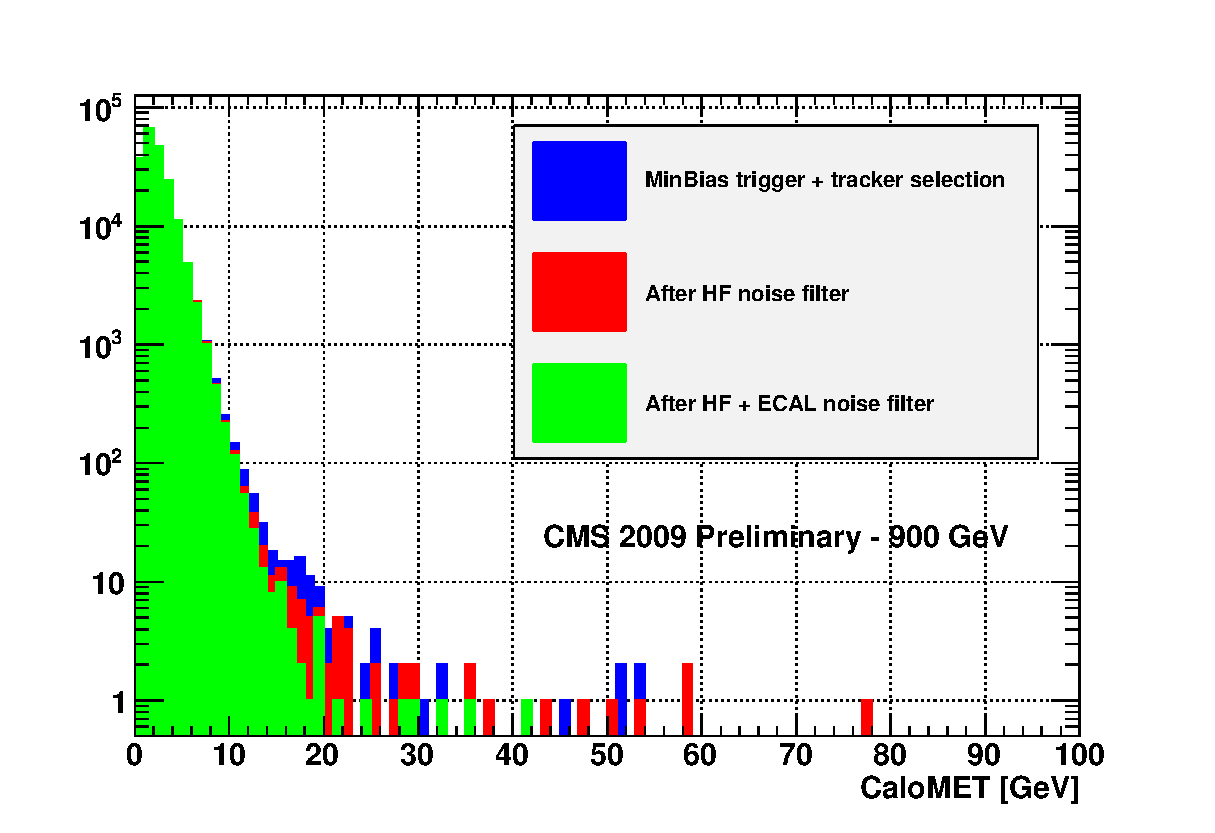
\includegraphics[width=0.5\textwidth]{plots_EventSelection/calometPt_afterFilters_900.eps} &
  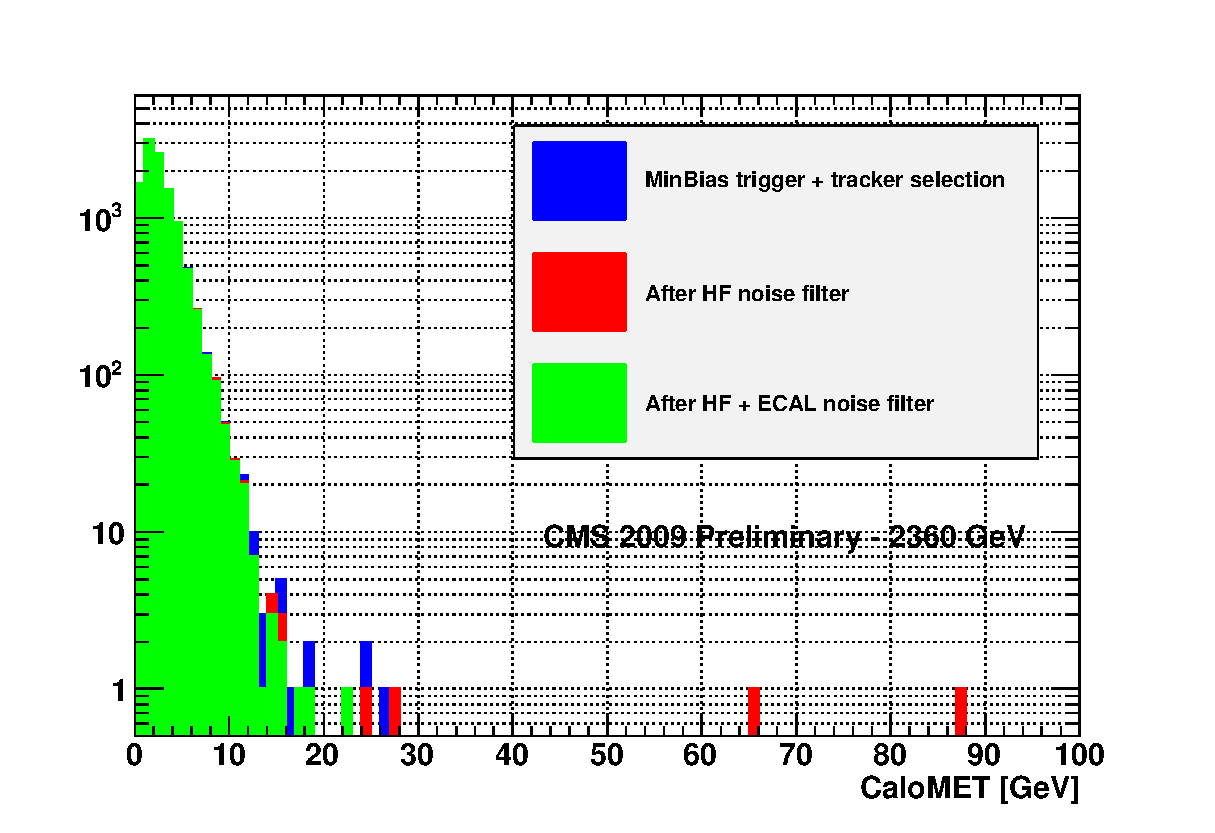
\includegraphics[width=0.5\textwidth]{plots_EventSelection/calometPt_afterFilters_2360.eps} \\
 \end{tabular}
 \caption{$\etmiss$ distributions in 900 GeV and 2360 GeV data after EB and HF noise cleaning}
\label{fig:calometAfterCuts}
\end{figure}


\section{Effects of Beam Halo Backgrounds}
\label{sc:BeamHalo}

The effects of machine-induced backgrounds, often referred to as beam halo, can be quite detrimental to $\etmiss$ or $\etmiss$-related quantities.  Figure~\ref{fig:BH_EventDisplay} shows a visualization of such an event, recorded during collision Run 123893~\footnote{ Run 123893 is not considered in the ``good'' run list as the Silicon Tracker was not participating in the run.}. Fortunately, lessons learned from prior collider experiments motivated an intense effort to identify beam halo and preclude its potential harmful effects to the $\etmiss$ observable.  To this end, several strategies and algorithms have been consolidated into a common framework known as the \verb BeamHaloId  package, which is still under active development.  The prototype version is executed during the standard reconstruction sequence as of \verb CMSSW_3_4_1 .   
  
\begin{figure}[htp]
\begin{center} 
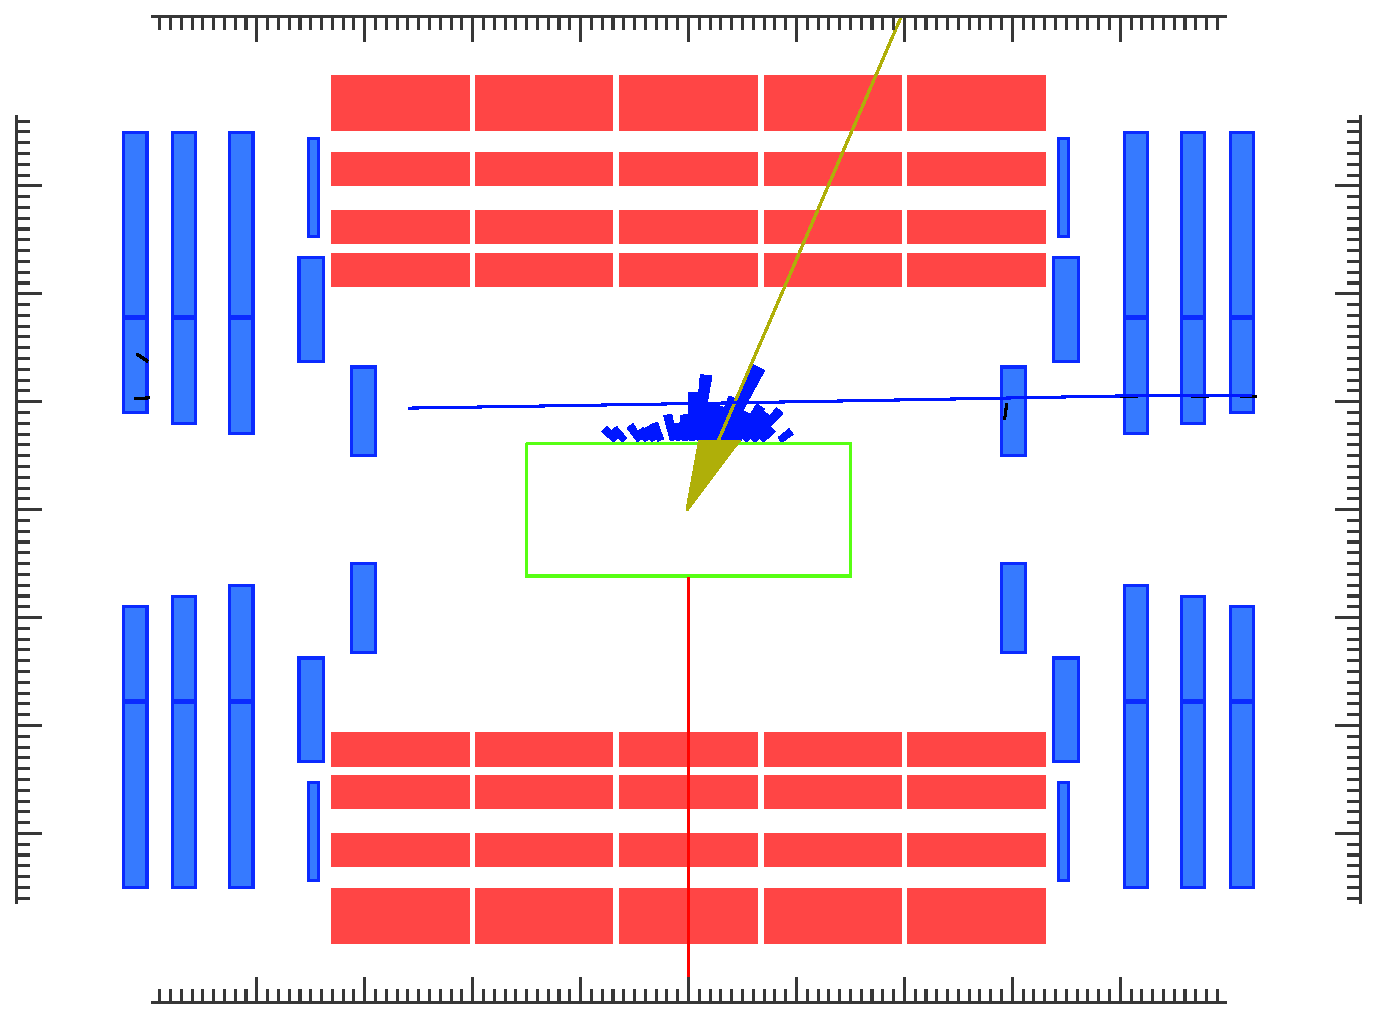
\includegraphics[scale=0.5]{plots_BeamHalo/Run123893_Lumi42_12070813_RZ.eps}
\end{center}
\caption{Event 12070813, Lumi Section 42 from collision Run 123893.  A halo muon track is shown in the CSCs (cyan) and extrapolated into the hadron calorimeter.  In this event the halo muon traversed several scintillators in a small $\phi$ window in the HCAL, yielding $\etmiss$ = 59.4 GeV (CaloMET) which is illustrated by the red vector pointing opposite to the energy deposits (blue) in the Hadron Calorimeter. A calorimeter jet (yellow) is also reconstructed in this event.  The BeamHaloId tools aspire to identify these types of events by combining information from the calorimeters and the CSCs. }
\label{fig:BH_EventDisplay}
\end{figure}

The \verb BeamHaloId  package is primarily designed to identify beam halo candidates which have trajectories pointing towards the barrel or endcap calorimetry. These are the most dangerous if one considers how the calorimeter-based $\etmiss$ overvable is constructed, i.e., via a negative vector sum over the transverse energy components of the calotowers.  Because beam halo particles are expected to have mostly parallel-to-beam trajectories, any interactions with the CMS calorimeters are very likely to occur along a narrow window in $\phi$.  Energy deposits in this pattern will conspire to maximally contaminate the magnitude of the $\etmiss$ vector, in contrast to a scenario where they are randomly distributed in $\phi$ allowing for some cancellations to occur. Of course, other MET algorithms which rely on the calorimetry are susceptible to beam halo as well.  

In order to best identify beam halo, information from three subdetectors is used in both a stand-alone and global way. Ecal and Hcal topological signatures, as well as time-of-flight information,  are used to identify halo at the rechit level.  The granularity of the Ecal also allows for observables based on shower shapes to be employed in the identification of beam halo.  This information from the calorimeters is combined with information from the CSCs (Cathode Strip Chambers)  to identify halo in a global way, as the CSCs are designed to be extremely efficient at measuring muons.  Because beam-induced muons can traverse the entire longitudinal dimension of the CMS detector in the span of 3 bunch-crossings, some inefficiencies are exptected in the CSCs at the reconstruction level.  Nonetheless, if the halo particles are charged, it is probable that they will leave enough hits in  a single endcap (either upstream or downstream) to allow for a stand-alone cosmic track to be reconstructed with beam halo-like kinematics.  This is especially important if the halo particles hit the calorimetry, as the CSCs provide nearly full geometrical coverage of barrel and endcap calorimetry in the transverse plane. 

There is even a dedicated Level-1 beam halo trigger implemented in the CSC Track Finder.  This trigger exploits the basic kinematic properties of beamhalo, imposing a tight $\delta$($\phi$) window and a minimum $\delta$($\eta$) requirement on two LCTs (local charged tracks) in CSC stations 1 and 2 or 1 and 3. The details of this trigger can be found in~\cite{ref:HaloTrig}. %CMS IN-2008/041, by D. Acosta, et al.

In order to commission the \verb BeamHaloId  tools in data, a pure sample with high statistics is needed. The CSC beam halo trigger is very useful for this purpose.  Unfortunately, most of the single-beam commissioning runs of 2009 did not feature CSC station ME1/1, which is the station closest to both the calorimeters and the beam line. This station is anticipated to get the most halo flux, but was often kept in standby mode in order to safeguard the hardware and electronics from beam splash events.  As a result, not many genuine beam halo events were triggered during these commissioning runs, and the BeamHaloId algorithms, especially those which serve to identify beam halo in the calorimeters, are not yet commissioned.

Despite the limited success with the single-beam commissioning runs, a small number of events was gleaned from the good collision runs (which featured station ME1/1) via the CSC beam halo trigger.  Because the cosmic background contamination to the CSC beam halo trigger is about 0.6 Hz, a requirement on the BPTX technical trigger was also imposed.  An event containing these two triggers in coincidence is defined as containing a beam halo particle.  Given that there are 3564 possible bunch crossings (or spacings) per orbit, the rate for a cosmic to fake a CSC beam halo trigger and coincide with BPTX trigger bit 0, can be estimated as:

\begin{eqnarray}
R_\text{fake} = \frac{(0.6\text{ Hz})\times N_\text{BX}}{3564}
\end{eqnarray}
where $N_\text{BX}$ represents the number of filled, colliding bunches per orbit. It is assumed the BPTX trigger bit 0 operates with 100\% efficiency.  This fake rate becomes $1.64 \times 10^{-4}$ Hz , $3.28 \times 10^{-4}$ Hz, $4.93 \times 10^{-4}$ Hz for 1, 2, and 3 colliding bunches per orbit respectively. 
  
Table~\ref{tab:BHStats} gives the beam halo statistics for each good collision run taken from the \verb PhysicsMuonBkg  Primary Dataset.  There were a total of 246 beam halo events identified during the good collision runs. Of these, 8 events were observed to pass the BSC event selection, indicating that a minimum bias collision occurred in the event.  Upon evaluating these 8 events with the help of an event display, it is clear that the beam halo triggers were faked by real collision muons.  This is an expected effect as some soft muons with forward trajectories can mimic a halo and thus satisfy the conditions of the L1 CSC beam halo trigger.  The $\delta$($\eta$) requirement used by this trigger was also loosened prior to the collision runs to accumulate more halo statistis for alignment purposes, therefore slightly enhancing the probability for a collision muon to pass the beam halo trigger.   
     
\begin{table}[h]
\begin{center}
\begin{tabular}{|c|c|c|c|c|} \hline
\multicolumn{5}{|c|}{L1\_SingleMuBeamHalo \&\& BPTX Bit 0 }    \\ \hline
 Run    & Colliding BXs & Lumis &  Events  & Rate [Hz]  \\ \hline 
123596  &  2  & 144&  1  & 7.5e-05 \\ \hline 
123732  &  2  & 99 &  9  & 9.9e-04 \\ \hline
123815  &  2  & 9  &  4  & 2.4e-03 \\ \hline 
123818  &  2  & 41 &  2  & 4.8e-04 \\ \hline 
123908  &  1  & 27 &  2  & 7.9e-04 \\ \hline 
124008  &  3  & 2  &  0  & -- \\ \hline 
124009  &  3  & 68 &  23 & 4.4e-03 \\ \hline 
124020  &  3  & 98 &  18(17)  & 2.0(1.9)e-03 \\ \hline 
124022  &  3  & 152&  48   & 3.4e-03 \\ \hline 
124023  &  3  & 89 &  35   & 4.2e-03 \\ \hline 
124024  &  3  & 81 &  26(25)  & 3.4(3.3)e-03 \\ \hline 
124025  &  3  & 13 &  2    & 1.7e-03 \\ \hline 
124027  &  3  & 35 &  20(18)  & 6.1(5.5)e-03 \\ \hline 
124030  &  3  & 31 &  11(9)  & 3.8(3.1)e-03 \\ \hline 
124120* &  1  & 57 &  45(43)  & 9.6(9.2)e-03 \\ \hline 

\end{tabular}
\end{center}
\caption{Summary of beam halo statistics for good collision runs at $\sqrt{s}=900$~GeV ($2.36$~TeV). *Run 124120 featured $\sqrt{s}=2.36$~TeV. A lumisection is included if it features BPTX bit 0 operating at nominal rates (indicating both beams crossing) and the L1\_SinglMuBeamHalo trigger operating at a minimum of the cosmic rate (indicating the CSCs and Track Finder are active).  The numbers given in parenthesis denote the runs which had events passing the BSC requirements for a minimum bias collision.  These numbers represent the beam halo statistics after the minimum bias events which fake halos are removed.}
\label{tab:BHStats}
\end{table}

For most of the earlier runs, the rates calculated in Table~\ref{tab:BHStats} are consistent with the cosmic background.  For the later runs, the rates are higher by roughly an order of magnitude, which indicates the unambiguous presence of machine-induced backgrounds.    \\

With these limited statistics some meaningful distributions can still be made. Figure~\ref{fig:BH_CaloMET} shows the differential  CaloMET rate for these selected events.  A few events exist beyond $\etmiss \ge 10$ GeV, which implies that some halo muons are hitting the calorimeters. Figures~\ref{fig:BH_Radial} and~\ref{fig:BH_Phi} show the position of the halo muon in the CSCs at its point of closest approach with respect to the calorimeters.  This information is extracted from the innermost rechit from the  CSC stand-alone cosmic track (if there was one reconstructed in the event).  The cosmic track reconstruction algorithms are optimized to measure muons which do not come from the collision point.

Of these 238 pure beam halo events~\footnote{The events with collision muons faking beam halo are not considered in these calculations and figures } , 221 or 92.8\% had at least one~\footnote{In some cases the halo muon will leave enough hits in both plus and minus muon endcaps to allow for two separate tracks to be reconstructed.} CSC stand-alone cosmic track in them, while 15 or 6.3\% had segments.  One event had no track or segments, but had rechits in the CSCs, and one event had no reconstruction level activity at all in the CSCs, despite the existence of a L1 CSC beam halo trigger.  The events in the CaloMET tails in Fig~\ref{fig:BH_CaloMET} all had stand-alone cosmic tracks in them.  

One can easily convert these rates into probabilities for a halo event to occur for a given colliding bunch crossing. Taking the beam halo rate from Run 124027, which was the highest (per colliding bunch) for the 900 GeV runs, and assuming an orbit rate of 11245.78 Hz, one obtains the probability, $P$, for a beam halo event in a colliding bunch crossing:

\begin{eqnarray}
%P &=& \frac{3.8 \times 10^{-3}\text{ Hz}/\text{BX} }{11245.78 \text{ Hz}}  \\
P &=& \frac{1.8 \times 10^{-3}\text{ Hz}/\text{BX} }{11245.78 \text{ Hz}} \\
  &=& 1.6\times 10^{-7} /\text{BX}
\end{eqnarray}

This implies that roughly 1 in 6.25$\times$10$^{6}$ colliding bunch crossings or minimum bias events will overlap with a CSC-triggered beam halo event.  A similar calculation can be done for the 2.36 TeV run to yield a ratio of 1 in 1.22$\times$10$^{6}$ colliding bunch crossings or minimum bias events.
 
It will be important to measure and monitor these rates once the beam intensities increase along with the frequency of minbias events. The probability of contamination is negligible in the current set of collision runs. This may not be the case, however, in the future.  \\


\begin{figure}[htp]
\begin{center}
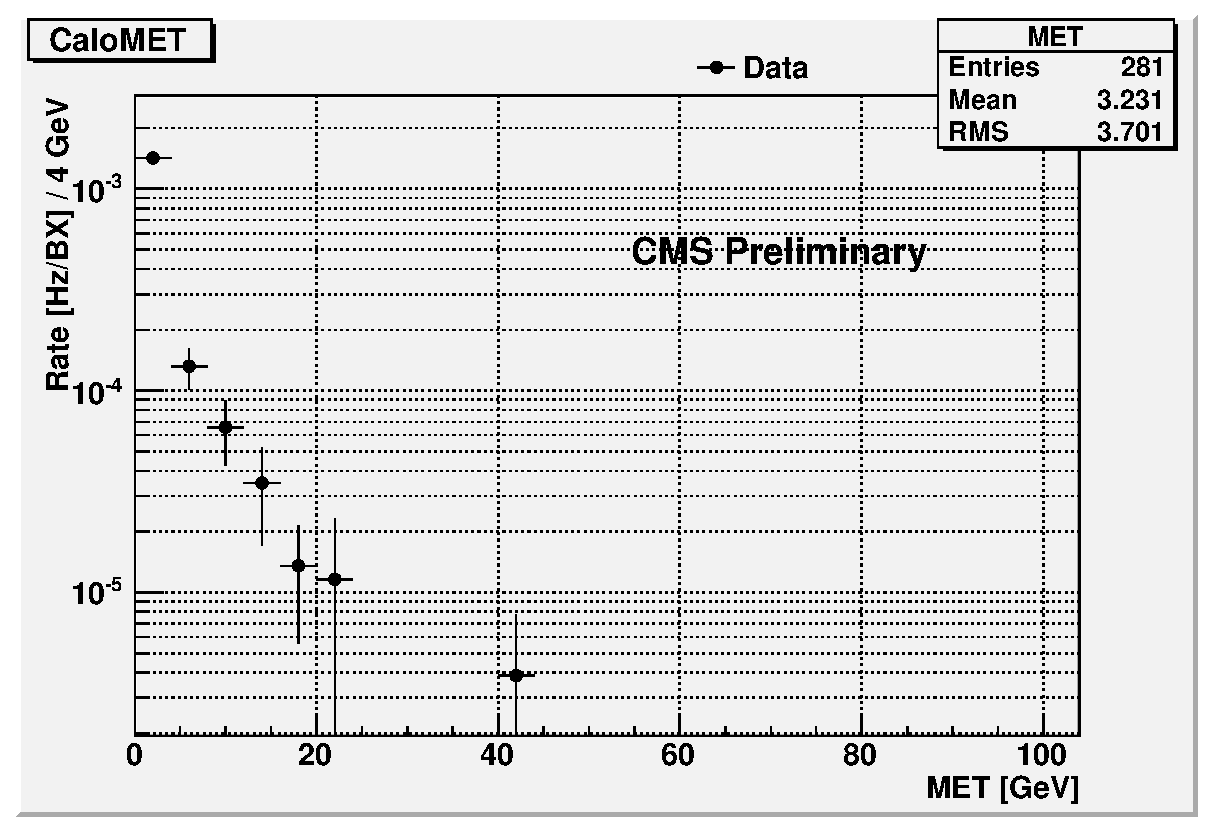
\includegraphics[scale=0.75]{plots_BeamHalo/CaloMET.eps}
\end{center}
\caption{$\etmiss$ differential rate distribution from the CSC beam halo AND BPTX triggered events recorded during the collision runs. Statistics were combined from each good collision run, including Run 124120 (2.36 TeV), and rates are normalized to a single bunch crossing.   }
\label{fig:BH_CaloMET}
\end{figure}

\begin{figure}[htp]
  \begin{center}
    \subfigure[Radial distribution of CSC halo tracks' impact point]{\label{fig:BH_Radial}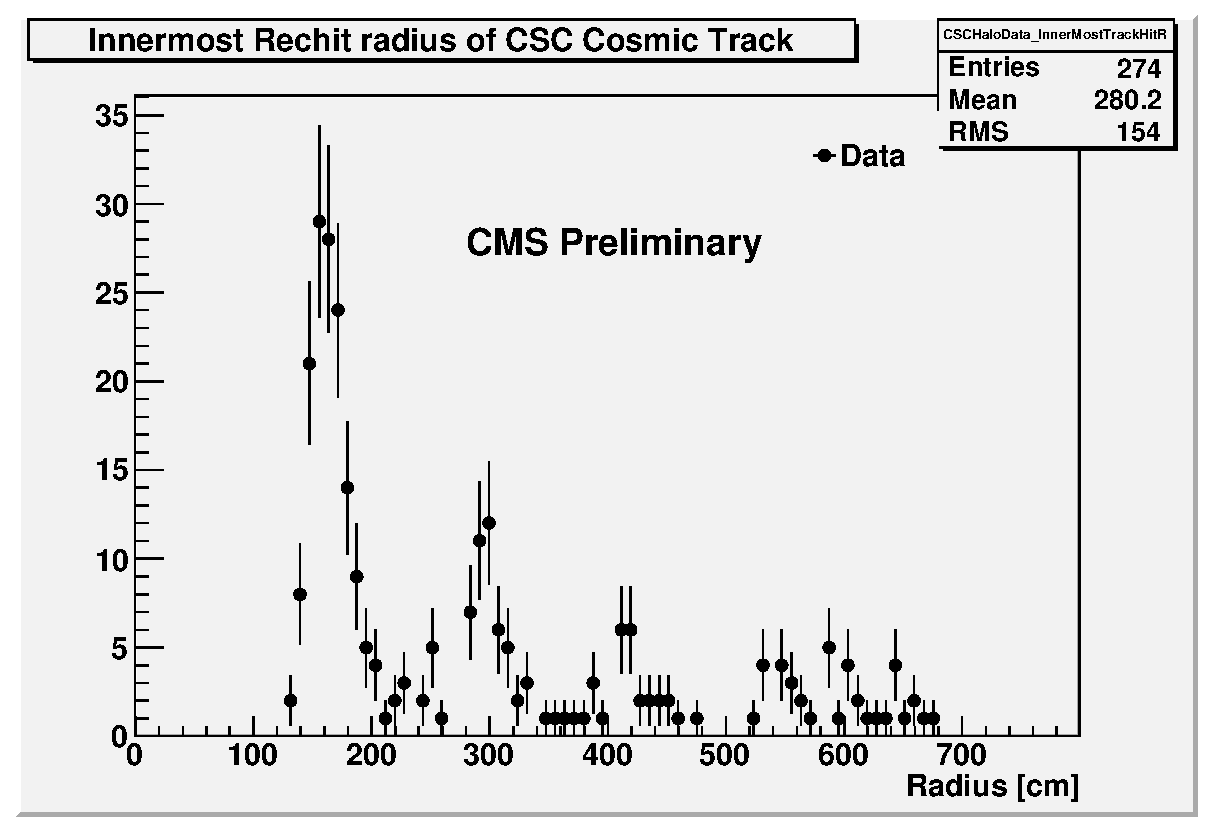
\includegraphics[scale=0.65]{plots_BeamHalo/InnerMostTrackHitR.eps}}
    \subfigure[$\phi$ distribution of CSC halo tracks' impact point]{\label{fig:BH_Phi}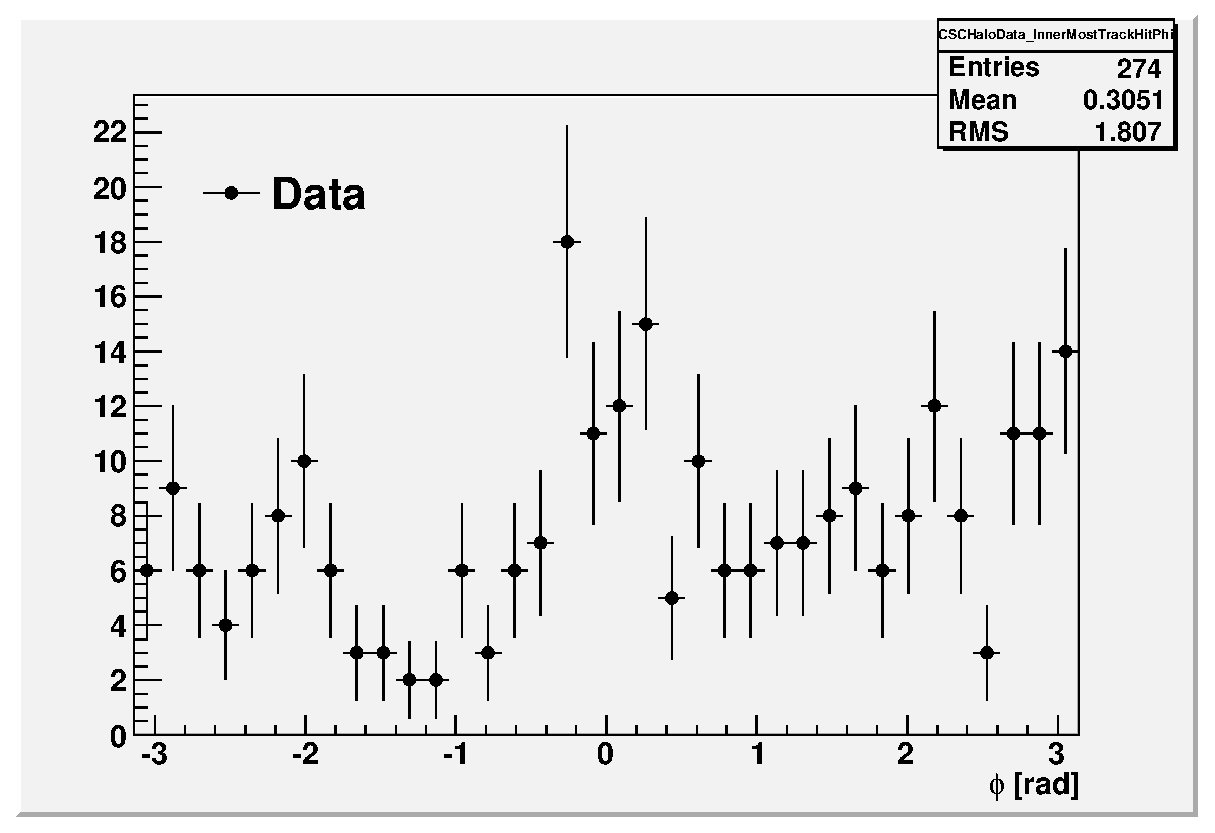
\includegraphics[scale=0.65]{plots_BeamHalo/InnerMostTrackHitPhi.eps}}
    \end{center}
  \caption{Global position of the constituent rechit of CSC stand-alone cosmic tracks at point of closest approach with respect to the calorimetry. Note: the  ECAL Barrel spans a radius from roughly 140 cm to 190 cm, while the Hcal Barrel spans roughly from 200 cm to 300 cm. The beam halo flux is expected to decrease as a function of radius. } 
  \label{fig:BH_ImpactPoint}
\end{figure}




\clearpage

